

\section{Etude fonctionnelle}

La solution logicielle que nous allons implémenter doit intégrer plusieurs scénarios de fonctionnement. Ceux-ci permettront de tester les aptitudes du patient en rééducation dans un contexte banal. Ces scénarios sont axés sur l'interaction entre le patient et le monde extérieur, via le "Domophone". 

\subsection{Scénario 1: Appel téléphonique entrant}

Le premier scénario à implémenter est assez basique. Il s'agit du cas où le résident reçoit un appel téléphonique. Il doit alors décrocher puis raccrocher le téléphone au terme de la conversation.

D'un point de vue logiciel, il s'agira de déclencher la sonnerie du téléphone pour avertir l'utilisateur. Une icône de téléphone peut être affichée en bas de l'écran, dans un coin. Ensuite, l'utilisateur devra se déplacer ver la zone du téléphone. Suivant le mode d'utilisation, le rendu sera différent : En mode symbolique, le logiciel basculera sur une vue du téléphone donnera les instructions pour décrocher puis pour raccrocher. En mode assisté, le téléphone sera en surbrillance et si l'utilisateur met trop de temps pour agir sur le téléphone, certains boutons peuvent se mettre en surbrillance ou clignoter.

\subsection{Scénario 2: Visite de l'infirmier}

Ce scénario correspond à la visite d'une personne connue par le résident. Lorsque que le visiteur arrive, il utilise l'interphone pour demander l'ouverture du portail. Le patient en rééducation doit décrocher le domophone, activer l'ouverture du portail grâce aux interrupteurs et raccrocher. Ce cas correspond bien à la visite d'un infirmier ou d'une quelconque personne que le résident peut reconnaître par la voix. 

Pour cette implémentation la différence avec le scénario 1 portera sur l'ouverture du portail. En effet, après avoir raccroché, l'utilisateur devra se rendre au niveau des interrupteurs et déclencher l'ouverture du portail. En mode symbolique, le basculement entre les vues sera automatique. Le mode assisté mettra en évidence l'ensemble des interrupteurs, puis en cas d'hésitation, le bon interrupteur sera mis en valeur.

\subsection{Scénario 3: Visite d'un inconnu}

Le scénario le plus complet correspond au passage d'un visiteur inconnu. En effet, le résident devra dans cette situation décrocher le téléphone, puis activer l'affichage vidéo de l'interphone sur l'écran de télévision de l'appartement. Ensuite, il devra vérifier qu'il peut laisser entrer le visiteur et le cas échéant, lui ouvrir le portail grâce aux interrupteurs, puis raccrocher. S'il ne désire pas lui ouvrir, il lui faudra juste raccrocher.
Ce scénario convient à plusieurs situations courantes : visite d'un réparateur, d'un livreur, d'un témoin de Jéhovah ...

Pour réaliser la partie "`visio TV"' de ce scénario l'utilisateur va devoir : activer la vision via le domophone, allumer la télévision et éteindre la télévision. Là encore, les 3 modes de fonctionnement vont modifier le comportement du logiciel et orienter plus ou moins l'utilisateur vers la télévision. En mode symbolique, l'utilisateur sera guidé pas à pas pour : 
\begin{itemize}
	\item activer la visio depuis le domophone
	\item allumer la télévision
	\item éteindre la télévision
\end{itemize}
La suite du scénario reprend le fonctionnement final du scénario 2, qui lui-même reprend la fin du scénario 1.

\subsection{Diagramme des cas d'utilisation}
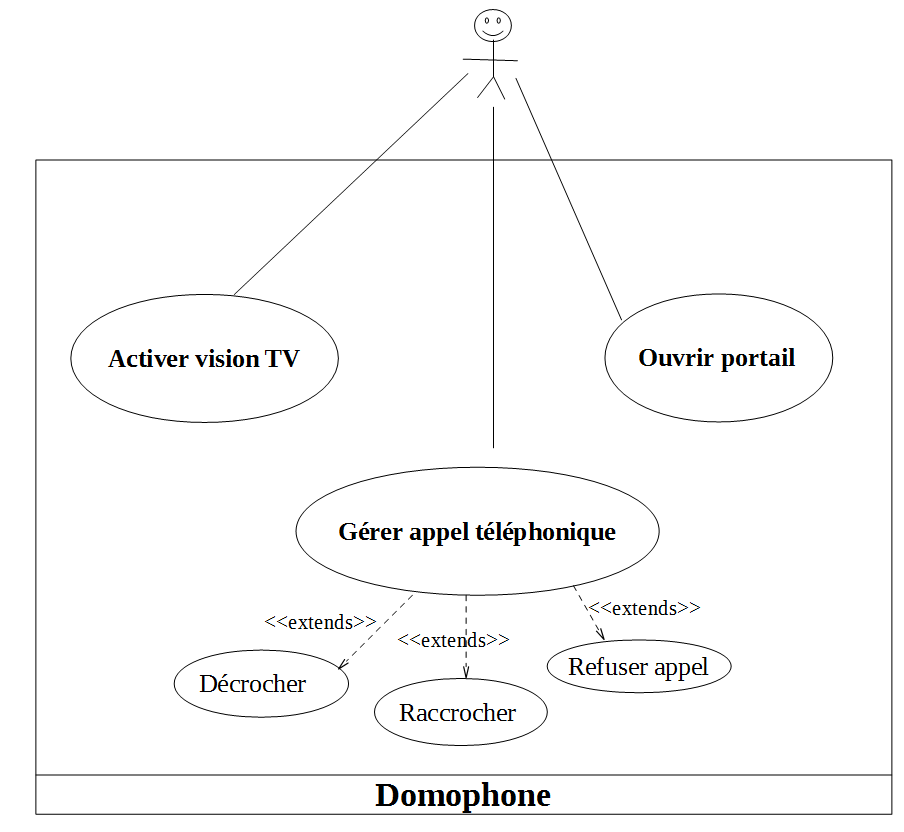
\includegraphics[scale=0.5]{1-PreEtude/img/use_case_diag}
